\documentclass[letterpaper, 10 pt]{report}

% For handling graphics
\usepackage{graphicx}
% For colors
\usepackage{color}
% For hyperlink
\usepackage{hyperref}
\hypersetup{
    colorlinks,
    linktoc=all,
    citecolor=black,
    filecolor=black,
    linkcolor=black,
    urlcolor=blue
}
% For mathematics
\usepackage{mathtools}
\usepackage[margin=1.0in]{geometry}

% -------------------------------------------------------------------------------------
% TITLE PAGE
% -------------------------------------------------------------------------------------
\begin{document}
\begin{titlepage}
\center
% Headings
\textsc{\LARGE Georgia Institute of Technology}\\[1.5cm]
\textsc{\large Center for Robotics \& Intelligent Machines}\\[0.5cm]
\textsc{\large Humanoid Robotics Lab}\\[0.5cm]
% Title
\rule{\linewidth}{0.5mm}\\[0.4cm]
{\huge \bfseries GT Mission Manual}\\[0.4cm]
\rule{\linewidth}{0.5mm}\\[1.5cm]
% Author
\textsc{\normalsize M.X. Grey}\\
\textsc{\normalsize Eric Huang}\\
\textsc{\normalsize Andrew Price}\\
\textsc{\normalsize Peter Vieira}\\[1.5cm]
% Image
\includegraphics[width=5.0cm]{resources/hubo-titlepage}
% Fill rest of page with whitespace
\vfill
\end{titlepage}

% -------------------------------------------------------------------------------------
% MISSION MANUAL
% -------------------------------------------------------------------------------------
\section*{Outline}
\begin{itemize}
\item List of code repos (ensure dependencing are included)
\item Installation instructions
\item Running instructions
\item Operation
\end{itemize}

\section*{Code Repositories}
\subsection*{ROS Code}
\begin{itemize}
\item hubo\_init
	\begin{itemize}
	\item \url{https://github.com/hubo/hubo\_init/}
	\end{itemize}
\item hubo\_walk
	\begin{itemize}
	\item \url{https://github.com/hubo/hubo\_walk}
	\end{itemize}
\item hubo\_motion\_ros
	\begin{itemize}
	\item \url{https://github.com/a-price/hubo\_motion\_ros}
	\end{itemize}
\item hubo\_manipulation\_planner
	\begin{itemize}
	\item \url{https://github.com/hubo/hubo\_manipulation\_planner}
	\end{itemize}
\end{itemize}
\subsection*{Real-time Code}
\begin{itemize}
\item hubo-ach
	\begin{itemize}
	\item \url{https://github.com/hubo/hubo-ach}
	\end{itemize}
\item hubo-motion-rt
	\begin{itemize}
	\item \url{https://github.com/hubo/hubo-motion-rt}
	\end{itemize}
\item hubomz
	\begin{itemize}
	\item \url{https://github.com/golems/hubomz}
	\end{itemize}
\end{itemize}

\newpage
\section*{Wall Drilling Task}

\subsection*{Procedure}
\begin{itemize}
\item 
\end{itemize}
\begin{center}
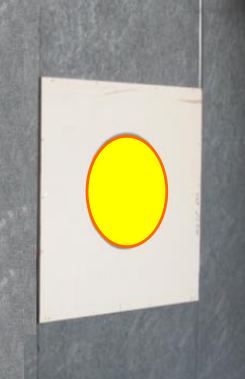
\includegraphics[width=8.0cm]{resources/wall-drilling}
\end{center}

\newpage
\section*{Rubble Clearing Task}
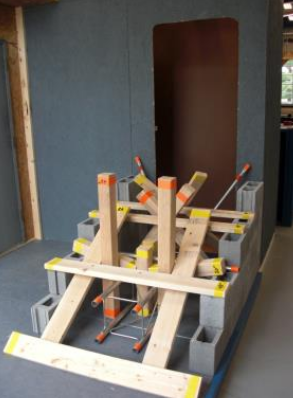
\includegraphics[width=8.0cm]{resources/rubble-clearing}


% -------------------------------------------------------------------------------------
% REFERENCES
% -------------------------------------------------------------------------------------
%\bibliography{}

% -------------------------------------------------------------------------------------
% END DOCUMENT
% -------------------------------------------------------------------------------------
\end{document}
